\documentclass{article}

\usepackage[utf8]{inputenc}
\usepackage{graphicx}
\usepackage{url}
\usepackage{color}
\usepackage{titlesec}
\usepackage{amsmath}
\usepackage{physics}
\usepackage{amsfonts}
\usepackage{subcaption}
\usepackage{booktabs}
\usepackage{hyperref}
\usepackage[counterclockwise]{rotating}
\graphicspath{{../figures/}}

\title{Paper draft v1.11 for supersat project}
\author{K. Latimer}
\date{June 25, 2021}

\newcommand{\drcomm}[1]{\textcolor{blue}{\textit{#1}}}
\newcommand{\klcomm}[1]{\textcolor{red}{\textit{#1}}}
\newcommand{\todo}[1]{\textcolor{green}{\textit{#1}}}

\begin{document}

\maketitle

\noindent\drcomm{Questions/comments from DR in blue} \\
\noindent\klcomm{Responses from KL in red}\\
\noindent\todo{Hanging details to address before final draft}\\

\section{Intro}

In a recent paper, Fan et al introduce a novel ``warm phase invigoration mechanism" (WPIM) in which increased concentrations of ultrafine aerosol particles (UAP$_{<50}$, with 50 signifying an upper bound on particle diameter of 50nm) in the boundary layer (BL) result in enhanced convective updraft speeds and precipitation rates \cite{Fan2018}. As pointed out by Grabowski and Morrison, the precise explanation for this physical effect is that, in allowing for lower equilibrium water vapor supersaturation (SS) values in rising convective parcels, these excess aerosol particles lead to an increase in the buoyancy of the parcel over the course of its ascent, thus enhancing convective speeds \cite{Grabowski2020}.

In order to get a quantitative intuition for how this works, we offer a simplified version of the calculation in \cite{Grabowski2015}, which still conveys the same essential idea. We consider a polluted (non-supersaturated; i.e. $RH=1$) storm ascending in an environment whose temperature profile has been set by clean storms. The parcel condenses water vapor as it rises, and for simplicity we assume no latent heat is lost to the environment. We then have (see Table \ref{vartable} for explanation of constants and variables used in the text. We use $\Delta$ here to represent a variation in state variables between two parcels, as distinguised from $d$ in Equation \ref{dCAPE} which denotes a proper differential form):
\begin{equation}
\label{energyconsv}
C_{ap}\Delta T + L_v\Delta q_v = 0,
\end{equation}
where $q_v$ is the water vapor mass fraction of the parcel ($q_v=m_v/m_{tot}$), also expressed in terms of the the relative humidity ($RH$) and saturation water vapor mass fraction ($q_v^*$) as:
\begin{equation}
\label{qveqn}
q_v = RHq_v^*
\end{equation}
Usig the Clausius-Clayperon equation:
\begin{align}
\label{clauclay}
\Delta q_v^* &= \Delta \Big(\frac{e_sV}{R_vTm_{tot}}\Big)\nonumber\\ 
&=\frac{\Delta e_s}{e_s}q_v^* - \frac{\Delta T}{T}q_v^*\nonumber\\ 
&=\frac{L_v\Delta T}{R_vT^2}q_v^* - \frac{\Delta T}{T}q_v^*\nonumber\\ 
&=\Big(\frac{L_v}{R_vT} - 1\Big)\frac{\Delta T}{T}q_v^*\nonumber\\ 
&\approx \frac{q_v^*L_v}{R_vT^2}\Delta T 
\end{align}
Taking the differential of Equation \ref{qveqn} and rearranging terms in Equations \ref{energyconsv}, \ref{qveqn}, and \ref{clauclay} yields:
\begin{equation}
\label{dT}
\Delta T = \frac{-L_vq_v^*}{C_{pa} + q_v\frac{L_v^2}{R_vT^2}}\Delta RH
\end{equation}
Plugging in typical values for $RH$ ($\approx 1.1$) and $T$ ($\approx 300$ K) gives $\Delta T\approx 1$ K.

In their paper (see for example Figure 2(b) of that work), Fan et al provide anecdotal evidence that the WPIM is capable of producing enhancements in vertical wind velocity on the order of 10 m/s for polluted relative to unpolluted storms. Even neglecting diffusive, frictional, or radiative losses, this requires a variation in convective available potential energy ($CAPE$) of $\approx 100$ J/kg, or a $RH$ difference between the dirty storm and clean environment of $\approx 0.1$, i.e., the environment must support SS on the order of 10\% throughout the troposphere.

While Fan et al do not offer any proof based on experimental data that such high SS exist in the convection setting the environmental lapse rate, they do observe comparable values in numerical simulations. In particular, using the Weather Research and Forcasting (WRF) model to simulate pristine (no UAP$_{<50}$) conditions in the Amazon Rainforest, they find (horizontally- and time-averaged) SS in convective cores of up to 15\%.

Since this is well above what is typically reported or assumed in the literature \cite{Hoppel1996, Yang2019, Koike2012, Politovich1988, Moteki2019, Siebert2017, Shen2018, Hammer2014, Li2019}, we seek in this paper to determine if we can find experimental evidence for O(10\%) SS in nature.

\section{Data Analysis and Results}

In order to determine experimental supersaturation within a reasonable margin of error, we must use the quasi-steady-state supersaturation ($SS_{QSS}$) formula \cite{Rogers1989}. In order to determine the region of validity for this approximation, we used data from the WRF output, since this allows us to compare to the true supersaturation (here called $SS_{WRF}$). We focused on the following considerations:
\begin{itemize}
\item The QSS approximation should be a good and reliable estimate for the actual SS, i.e. least-squares linear regression (LSLR) slope and correlation coefficients $\approx$1.  
\item We want the criteria to be inclusive enough that we are still capturing a significant fraction of the convection which sets the average temperature profile of the troposphere.
\item In keeping with the analysis by Fan et al, and with our general interest in studying convective cores, we additionally exclude the $w$ lower bound value of 0 to ensure we are capturing reasonably strong updrafts. 
\end{itemize}
In Figure \ref{filtcritheatmap} we synthesize the data needed to take all three of the above considerations into account. In order to make a quantitative comparison between various filtering criteria we define the following skill score based on the LSLR parameters for $SS_{WRF}$ vs $SS_{QSS}$, which is the Euclidean distance in the 4-dimensional space of tuples $(m_{poll}, R^2_{poll}, m_{unpoll}, R^2_{unpoll})$ from the ideal point $(1, 1, 1, 1)$:
\begin{equation}
\label{skillscore}
\text{Skill score } = \sqrt{(1-m_{unpoll})^2 + (1-R_{unpoll}^2)^2 + (1-m_{poll})^2 + (1-R_{poll}^2)^2}
\end{equation}
Here $m$ represents the LSLR slope and $R^2$ is the correlation coefficient, and subscripts `poll' and `unpoll' correspond to Fan et al's `C\_PI' (polluted) and `C\_BG' (unpolluted) model scenarios, respectively.

We find that taking $LWC > 10^{-4}$ kg/kg and $w>1$ m/s yields the best agreement of the QSS approxiamtion with the true SS while still yielding a subset of the data that accounts for greater than half of the condensational latent heating in the troposphere below the freezing line and consists of reasonably strong convective updrafts. To summarize, we use the following criteria in all subsequent analyses:
\begin{itemize}
	\item T \textgreater  273K (we're not including ice in the theory; note that Fan et al do evaluate SS wrt water above the freezing line though)
	\item w \textgreater  1 m/s
	\item cloud LWC \textgreater  1e-4 g/g (in the convection core) 
	\item including rain droplets and ventillation corrections
\end{itemize}
All points (whether in simulation or field campaign data) satisfying the first three conditions listed above are henceforth referred to as ``warm cloudy updrafts" or WCU. 

The LSLR on $SS_{WRF}$ versus $SS_{QSS}$ after applying the filtering scheme described above yields similar results for both the polluted and unpolluted cases (Figure \ref{wrfvsqss}). We therefore combine the datasets in order to define the predicted value $SS_{pred}$ of the true supersaturation based on the value of $SS_{QSS}$, which is the experimentally accessible quantity:
\begin{equation}
\label{sspred}
SS_{pred} \equiv m_{combined}*SS_{QSS} + b_{combined},
\end{equation}
where we find values of the regression parameters (labeled with the subscript `combined' to denote the combined polluted and unpolluted datasets) of $m_{combined}=0.83$ (unitless) and $b_{combined}=0.04$ (\%).

\begin{figure}[ht]
    \centering
    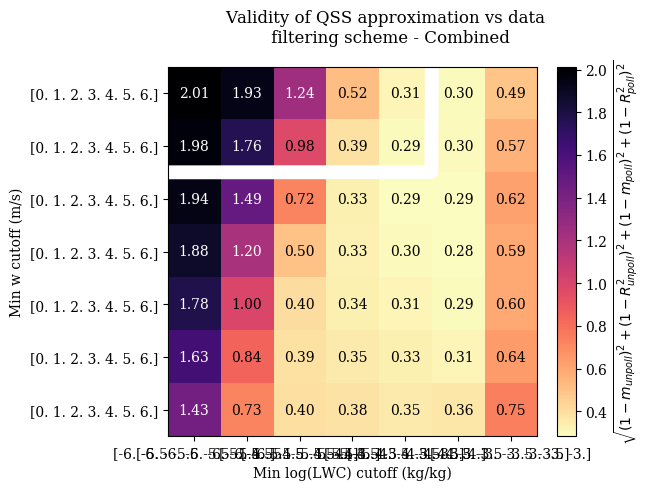
\includegraphics[width=9cm]{wrf/filtering_criteria_figure.png}
    \caption{Systematic evaluation of data filtering scheme using WRF model outputs. Here, the heatmap color corresponds to the value of the skill score (\ref{skillscore}) for each pair of cutoff values for liquid water content (horizontal axis) and vertical wind velocity (vertical axis). Numerical values of the skill score are also given as annotations to aid in distinguishing similar colors. In all cases we additionally restrict our consideration to points with temperature above 273 K. We also seek to evaluate the fraction of domain-wide positive (i.e. condensational) latent heating attributed to points selected through the data filter. The higher the fraction, the more confidence we have (in an unquantified sense) that we are capturing a complete picture of the convection which sets the temperature profile in the troposphere. Grey hatching indicates the region of the heatmap where the LH fraction is $< 50\%$ for both polluted and unpolluted model scenarios.}
    \label{filtcritheatmap}
\end{figure}

We would like to further quantify the spread of true SS values for a given value predicted by the QSS approximation. In Figure \ref{ssquantiles}, we plot a range of quantiles for the true SS given the predicted SS, using the polluted and unpolluted data sets combined.% (see Table \ref{lsrtable} for details on the regression parameters for each case). 
\begin{figure}[ht]
	\centering
	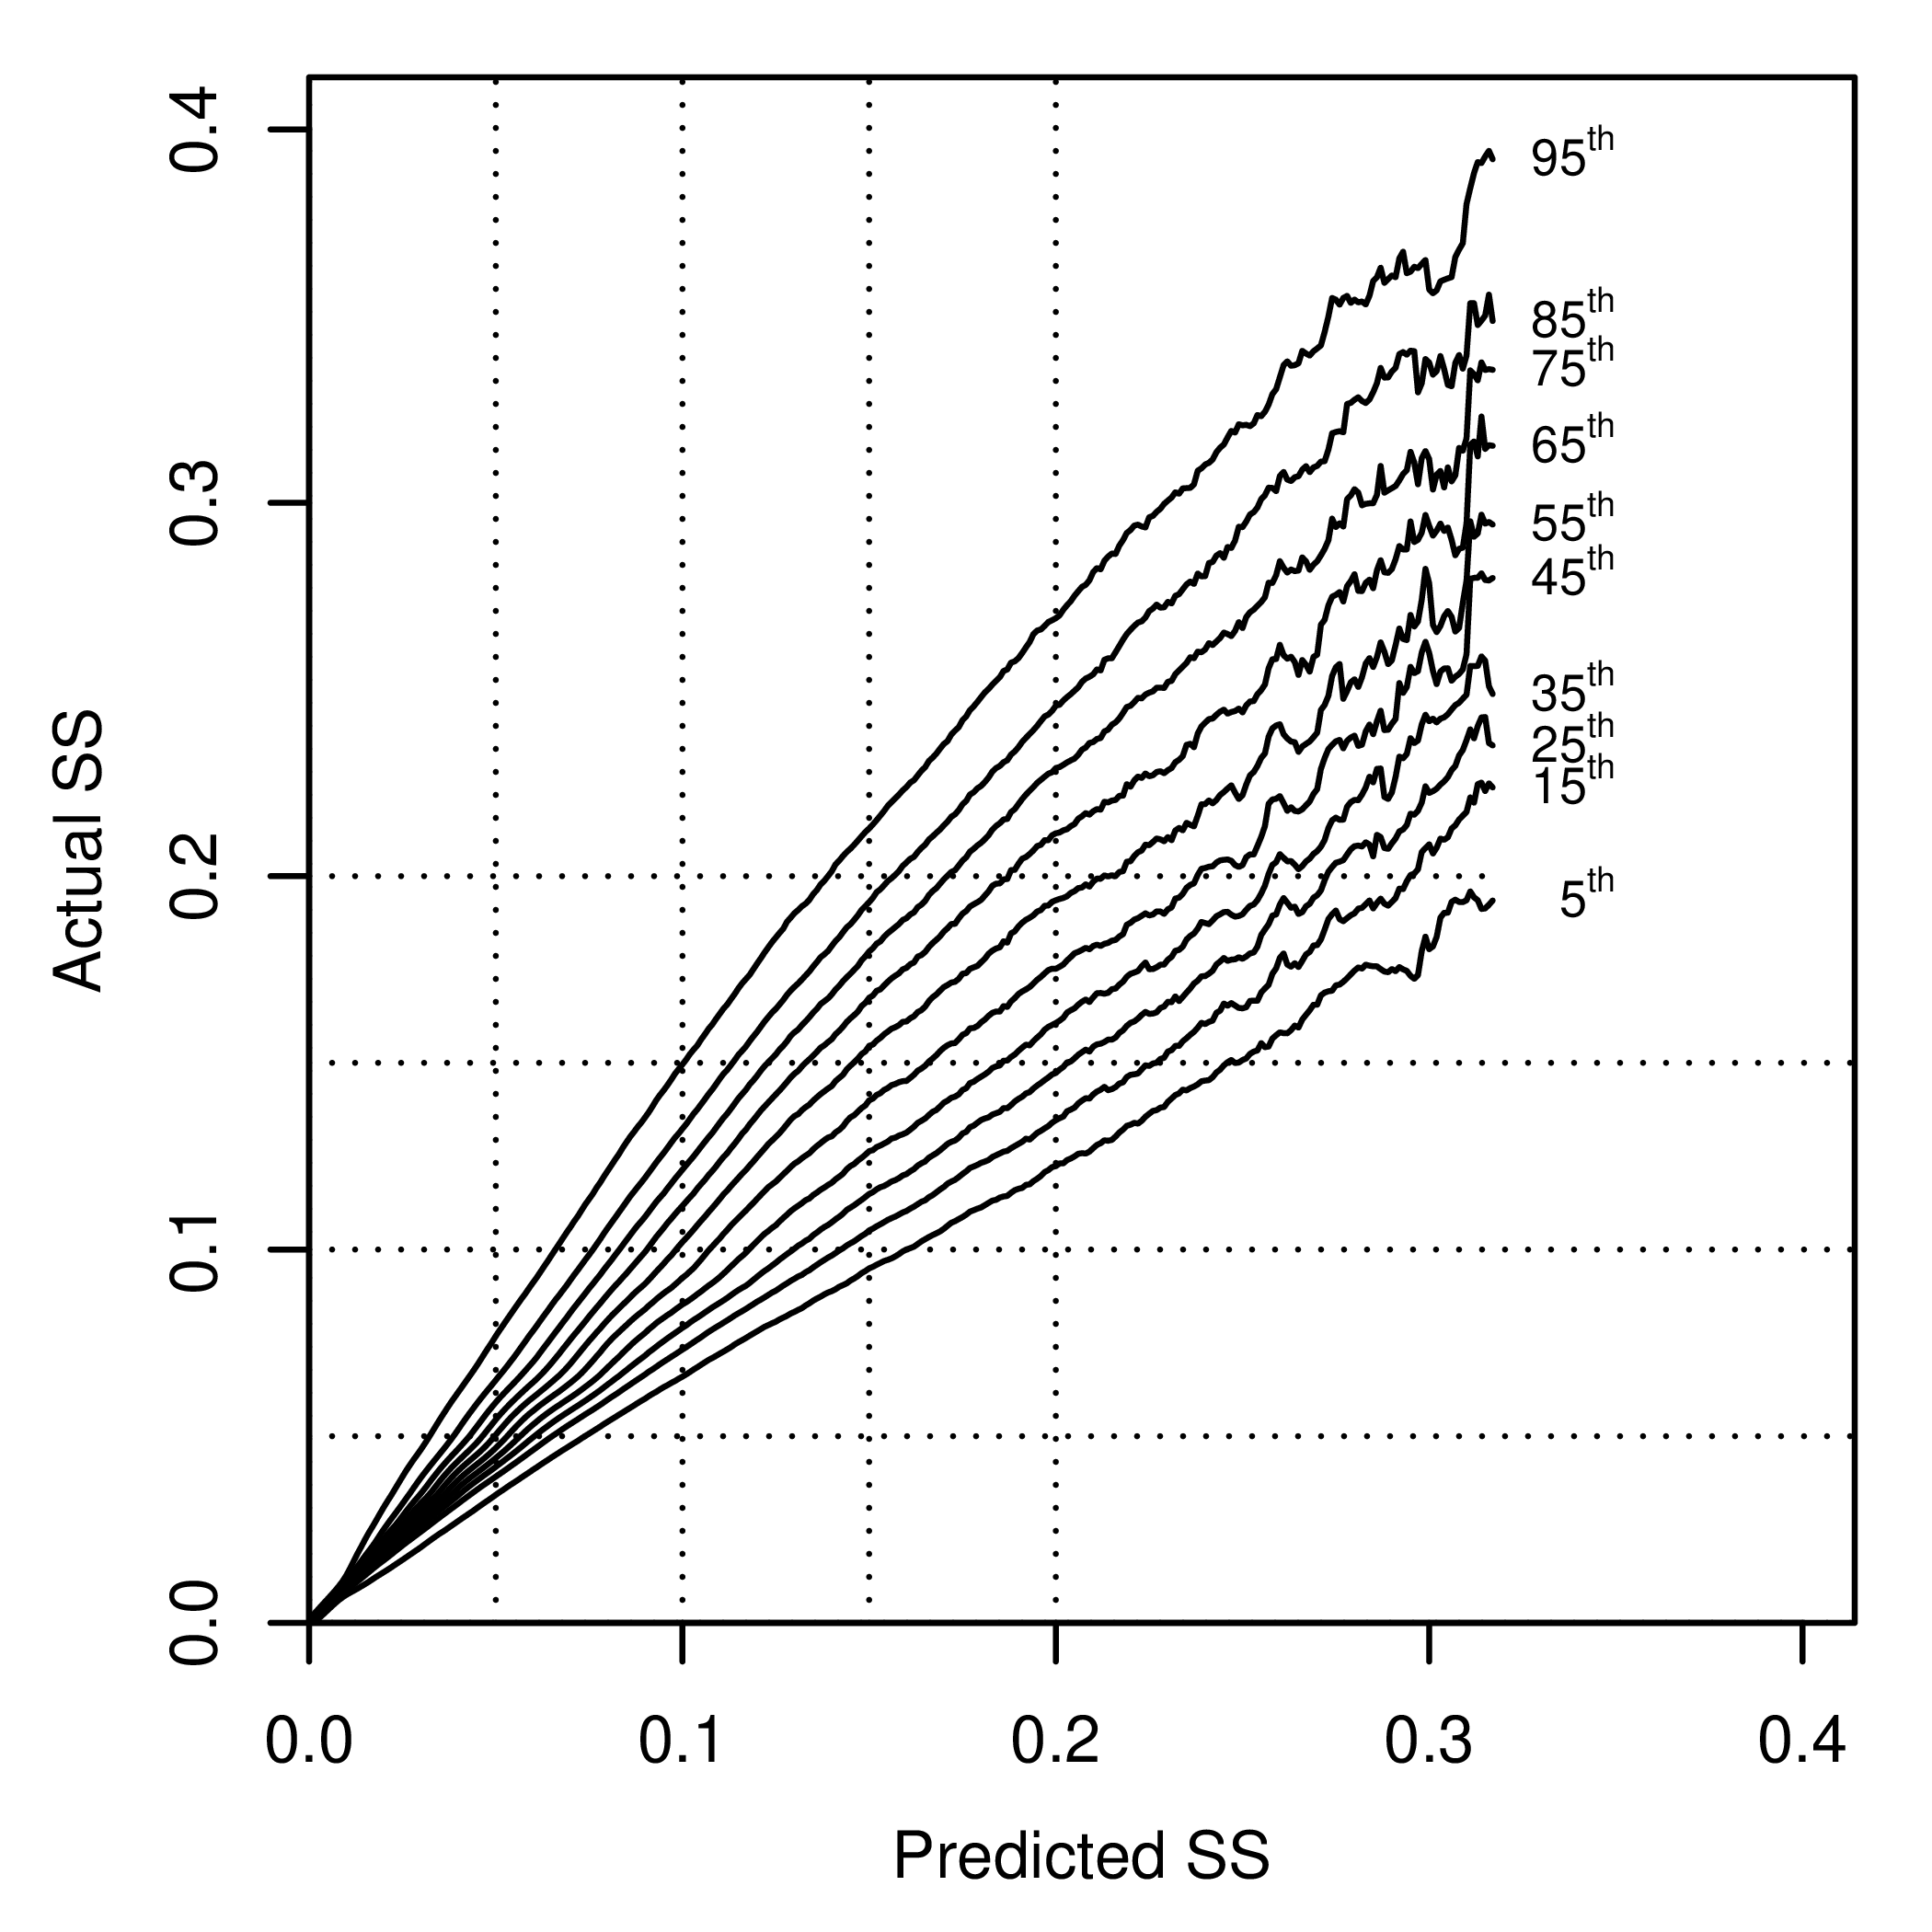
\includegraphics[width=\textwidth]{wrf/18supersat_predict.png}
	\caption{This figure shows the spread of true SS values (i.e., those given in the WRF output) for a given value of supersaturation predicted using the derived value of $SS_{QSS}$ and Equation \ref{sspred}. Each curve follows a fixed quantile (labeled on the figure) across the domain of predicted SS values for the range of actual SS. The quantiles are calculated with a 0.01-wide moving window centered on the respective predicted value. We see that the actual SS hew closely enough to the predicted SS that a high predicted SS guarantees a high actual SS, and vice versa. Up to about a QSS SS of 0.1, the median actual SS is, to good approximation, equal to the predicted SS. From this plot we can simply read off the confidence level of our lower bound on actual SS; for example, for a single predicted SS of 0.1, there is 95\% confidence that actual SS $<$ 0.15.}
	\label{ssquantiles}
\end{figure}

In their analysis, Fan et al use the following filtering criteria:
\begin{itemize}
	\item For experimental data: They examine the upper 10th percentile of updrafts in ``convective events" which 1) Fall between 11h00 and 19h00 local time 2) Have no other convective events occuring at any point in time 3 hours prior, and 3) Have max echo height at $>$0dBz above 10km. For aerosol measurements they take the average of measurements in the 30-min interval prior to the convective event. The authors do not state their criteria for what qualifies as a convective event.
	\item For model data: They limit analysis to a subset of the horizontal domain (red box in Fig S8) that encompasses a single convective event during the day of the simulation. They again take the top 10th percentile of updrafts with $w>2$. 
\end{itemize}

Because we use slightly different filtering criteria than that described above, we first verify that the data points selected by our filter yield similar SS profiles in the WRF simulation as those found in the latter work. In Figure \ref{wrfssvertprof} we plot vertical SS profiles for WCU, as well as for the top 10\% WCU. We define the points in the ``upper 10 percentiles" as those with $w$ greater than the 90th-percentile (out of all altitudes and times) vertical wind velocity, and we use the shorthand ``top 10\% WCU" to refer to this subset. Data in Figure \ref{wrfssvertprof} are binned according to the simulation grid. For this and future vertical profiles, the vertical coordinate of plotted points represents the average over all vertical coordinates of points in the corresponding bins. In \cite{Fan2018} they consider a restricted subdomain around the T3 field station, indicated in Figure S8 of the supplementary information for that paper; we do not see a major qualitative difference when including this additional criterion; see Figure \ref{wrfsubdomssvertprof}. We do indeed find the high SS values reported by Fan et al (maximum values of 13\% in both polluted and unpolluted cases from the upper 10th percentile dataset), confirming that our filtering criteria establish a fair basis for comparison here.

\begin{figure}[ht]
	\centering
	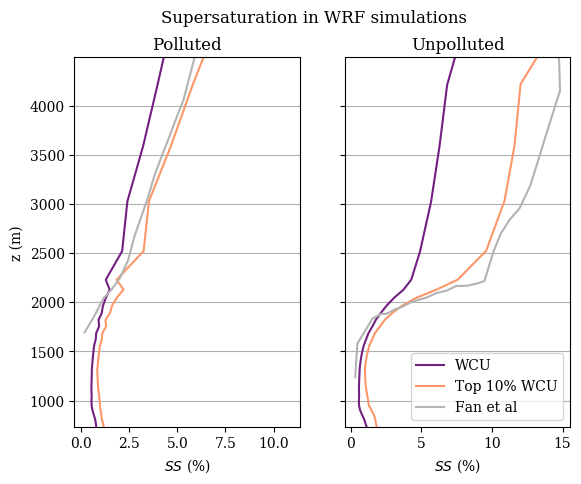
\includegraphics[width=\textwidth]{wrf/ss_pred_vs_z_figure.png}
	\caption{This figure serves to verify that our data filtering scheme yields SS profiles similar to those obtained by Fan et al (c.f. Figure 4 of that paper). Using WCU points (purple) and only the top 10 percentiles of WCU points as measured by $w$ (orange; see text for details), the latter being aligned with the analysis method of Fan et al. Profiles show $SS_{pred}$ averaged across time and horizontal spatial coordinates. Vertical grid is obtained by averaging over altitude values for each vertical layer in the simulation grid, which is based on pressure coordinates. In addition to imposing the filtering criteria described in the text, we only plot points in the vertical profile for which the area fraction occupied by WCU is greater than 0.01\%. The gray curves are digitized from Figure 4B of \cite{Fan2018}, and represent values of $SS_{WRF}$, i.e. the supersaturation values directly given in the simulation output rather than predicted from derived values of $SS_{QSS}$. We observe that our filtering scheme indeed recovers average $SS_{WRF}$ values on the order of 10\% as reported in \cite{Fan2018}.}
	\label{wrfssvertprof}
\end{figure}

\clearpage
\newpage

We now seek to determine whether such high values actually occur in nature. The experimental dataset we reference here comes from the Aerosol, Cloud, Precipitation, and Radiation Interactions and Dynamics of Convective Cloud Systems - Cloud Processes of the Main Precipitation Systems in Brazil: A Contribution to Cloud Resolving Modeling and to the GPM (Global Precipitation Measurement) (ACRIDICON-CHUVA) field campaign carried out in the Amazon Rainforest (Brazil) over a two-year period in 2014-15. Specifically, we analyze cloud and rain drop spectra collected on the High-Altitude Long-range Aircraft (HALO), a Gulfstream G550 equipped with several instruments to measure meteorological, chemical, microphysical, and radiative quantities \cite{Wendisch2016}. See the Methods section for further details. [\klcomm{I am open on how to structure this information throughout the paper; on the one hand maybe it's confusing to break things up but on the other hand it does feel slightly excessive to delve into all the minutiae in the main text?}] Figure \ref{halossvertprof} shows the analogue of Figure \ref{wrfssvertprof} using data from all HALO flight dates combined. We find no points with average SS above 1 \%, even when limiting to the strongest updrafts in the combined dataset.

\begin{figure}[ht]
    \centering
    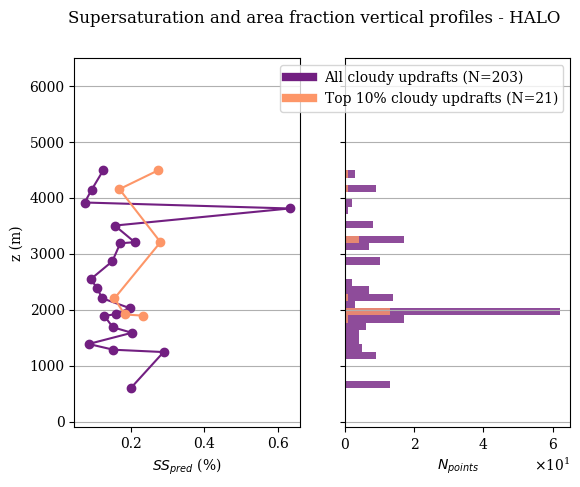
\includegraphics[width=9cm]{halo/ss_pred_vs_z_figure.png}
    \caption{This figure serves to determine whether the high-SS values found in the WRF simulation output indeed occur in nature. Profile shows $SS_{pred}$ averaged across WCU (purple) from HALO flight campaign (all dates combined), as well as across only top 10\% WCU (orange; see text for details). Vertical grid is evenly spaced throughout the same altitude range used for the WRF simulations (see caption of Figure \ref{wrfssvertprof}), with a $z$ interval of about 200m. We do not find any points in the $SS_{pred}$ profile with values above 1\%, even when restricting to only the top 10 percentiles.}
    \label{halossvertprof}
\end{figure}

We can use Equation \ref{dT} and the SS profiles in Figures \ref{wrfssvertprof} and \ref{halossvertprof} to infer a buoyancy profile for a hypothetical non-supersaturated parcel. For this analysis we take the temperature of the parcel equal to that of the environment (i.e., what has been measured). The resulting error in the value of $\Delta T$ in Equation \ref{dCAPE} is quadratic in $\Delta RH$, which is acceptable for our purposes. In Figure \ref{dTprofiles} we plot $\Delta T$ profiles from both WRF simulations and field campaigns side-by-side. We use these profiles to derive enhancements in $CAPE$ for the non-supersaturated parcel as:
\begin{equation}
\label{dCAPE}
\Delta CAPE = g \int dz \frac{\Delta T}{T}
\end{equation}
where we again approximate $T$ as the environmental temperature and integrate from 647 to 4488 m, the common vertical domain for all four curves in Figure \ref{dTprofiles}. We find values of $\Delta CAPE$ of 2, 25, and 50 J/kg for HALO, WRF (polluted), and WRF (unpolluted), respectively. Neglecting any other physical energy sinks as above, these translate to vertical velocity enhancements on the order of 1 m/s in the field campaign and 10 m/s in both the simulations under consideration.

\begin{figure}[ht]
    \centering
    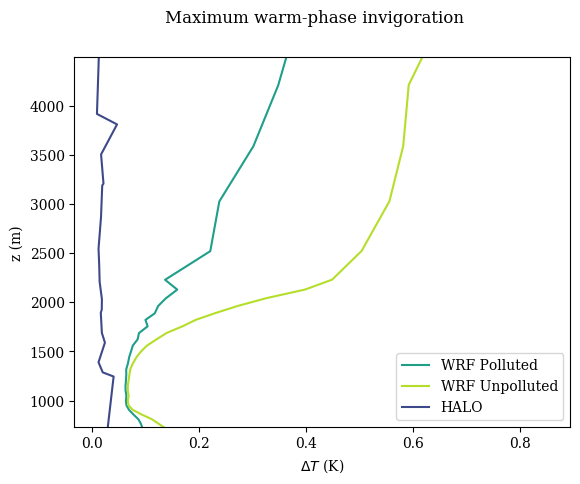
\includegraphics[width=12cm]{wrf/combined_dT_profile_figure.png}
    \caption{[\klcomm{I'm using different colors for polluted / unpolluted WRF simulations because different linestyles don't show up very well in the vertical wind velocity histogram}] Profiles for $\Delta T$ of a non-supersaturated ($RH=1$) parcel ascending in an environment with SS profiles for all WCUs shown in Figures \ref{wrfssvertprof} and \ref{halossvertprof}, using Equation \ref{dCAPE}. We find that the buoyancy of this hypothetical parcel in nature is far lower than in the simulations, casting doubt on the real validity of the WPIM as described in Fan et al.}
    \label{dTprofiles}
\end{figure}

One possible counterargument is that the aerosol concentrations in the BL during the dates of the HALO flights might have been significantly higher than those during the dates considered in Fan's paper, thus precluding the occurence of high SS values in the troposphere. In order to investigate this, we use the aerosol particle size distribution measured by the scanning mobility particle sizer (SMPS) in Manacapuru, located southwest of Manaus (PI: Chongai Kuang). This intrument measures particle concentrations in the diameter range 11.1-469.8nm. In Figure \ref{goamazonhist}, we show that, while we do indeed see higher total aerosol concentrations on average during the HALO flight date range (3500/ccm vs 2400/ccm), the UAP50 concentration is on average lower (670/ccm vs 1600/ccm). In fact, the aerosol concentrations used in the WRF simulations are much lower than those observed during the day the simulation takes place, which is not justified quantitatively in that study.

We note additionally that the positive experimental correlation between concentration of UAP50 and maximum vertical velocity during the dates studied by Fan et al is not significant at the 95\% confidence level - the LSLR slope parameter for their data set has a p-value of 0.11.
\begin{figure}[ht]
	\centering
	\begin{subfigure}{0.7\textwidth}
		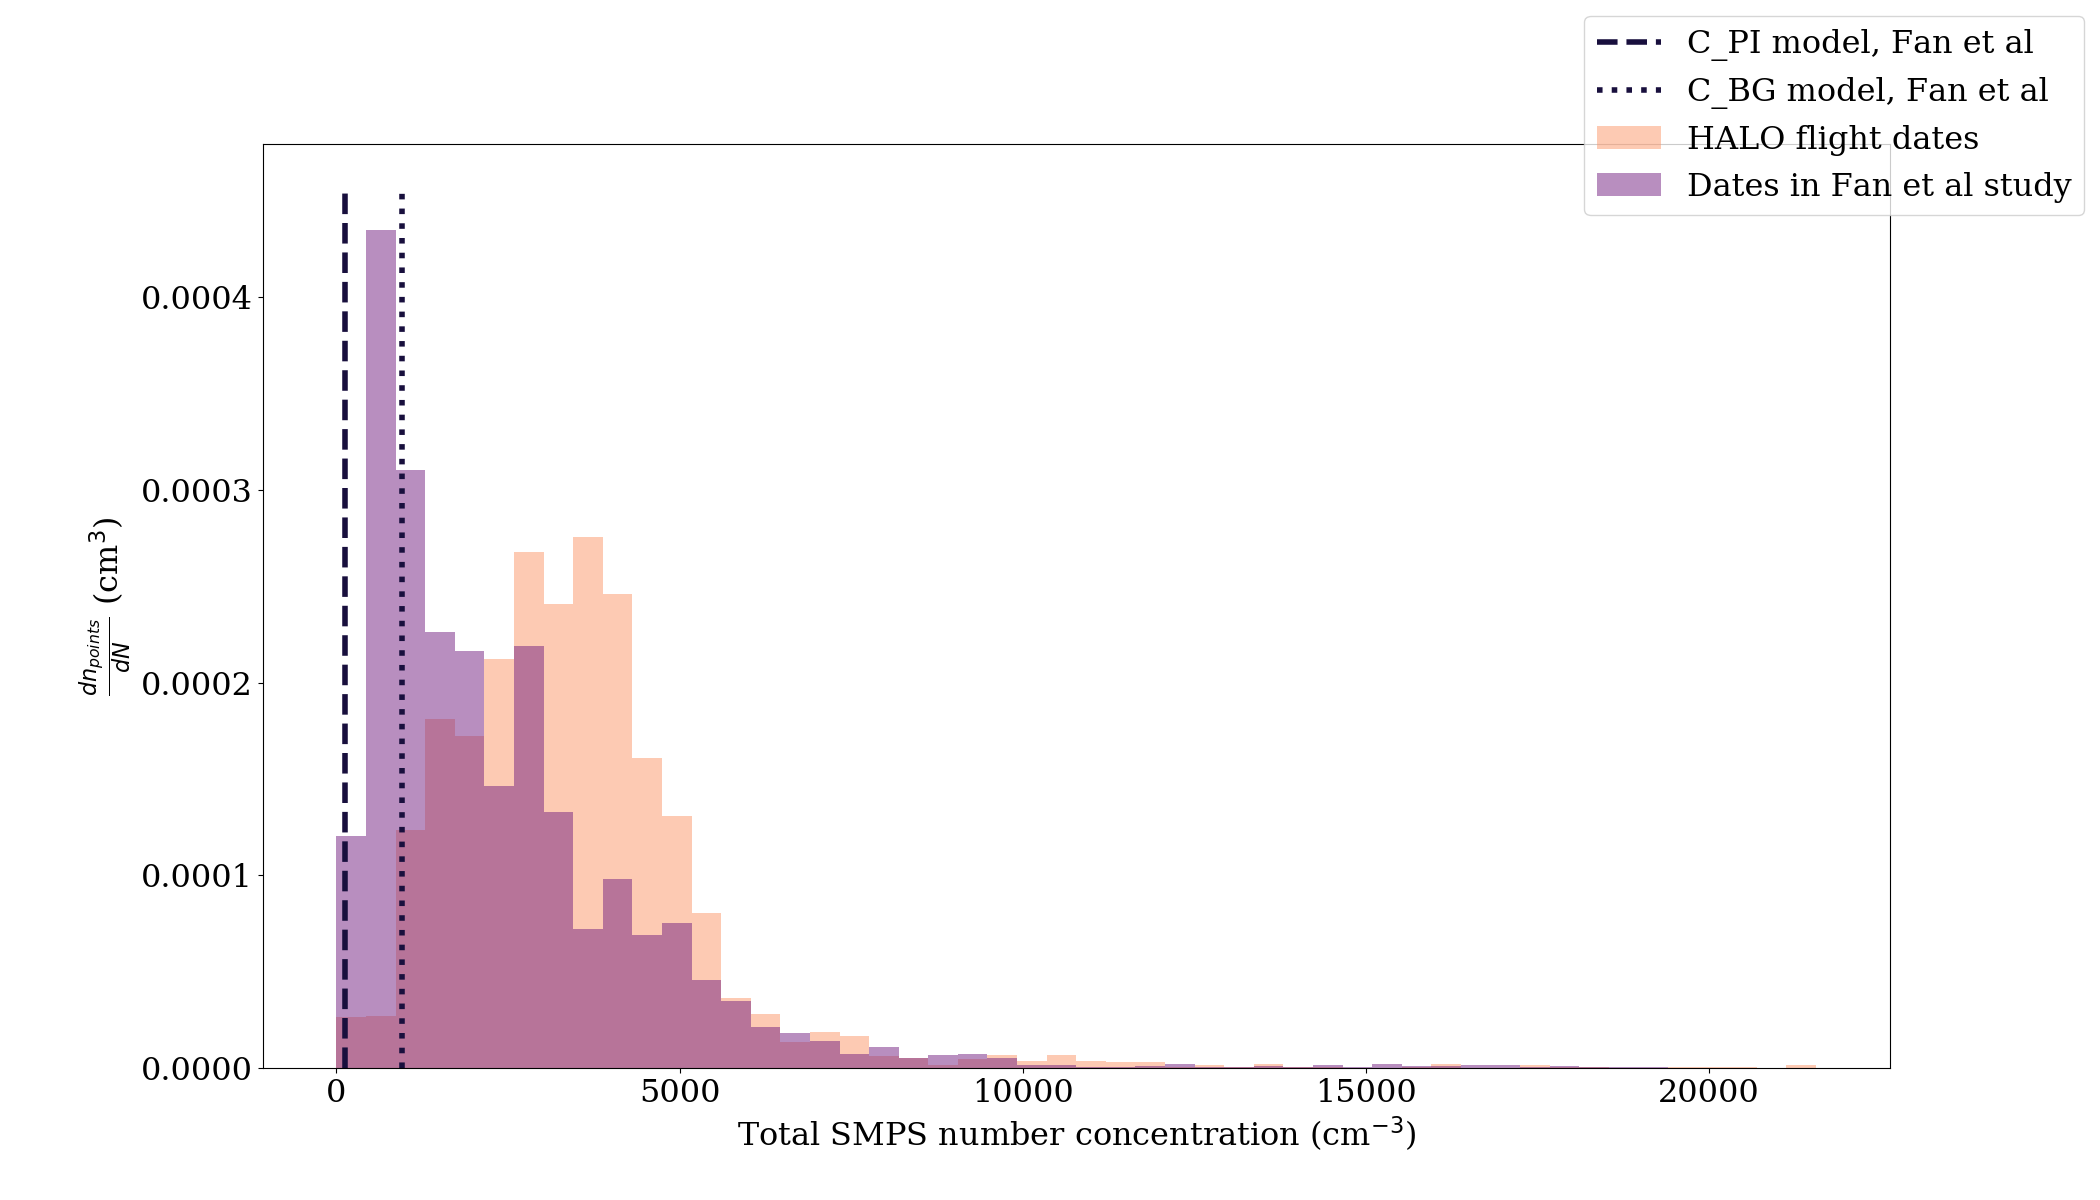
\includegraphics[width=\textwidth]{goama/v1_FINAL_tot_compare_nconc_hist_alldates_figure.png}
		\label{goamazontothist}
		\caption{}
	\end{subfigure}
	\begin{subfigure}{0.7\textwidth}
		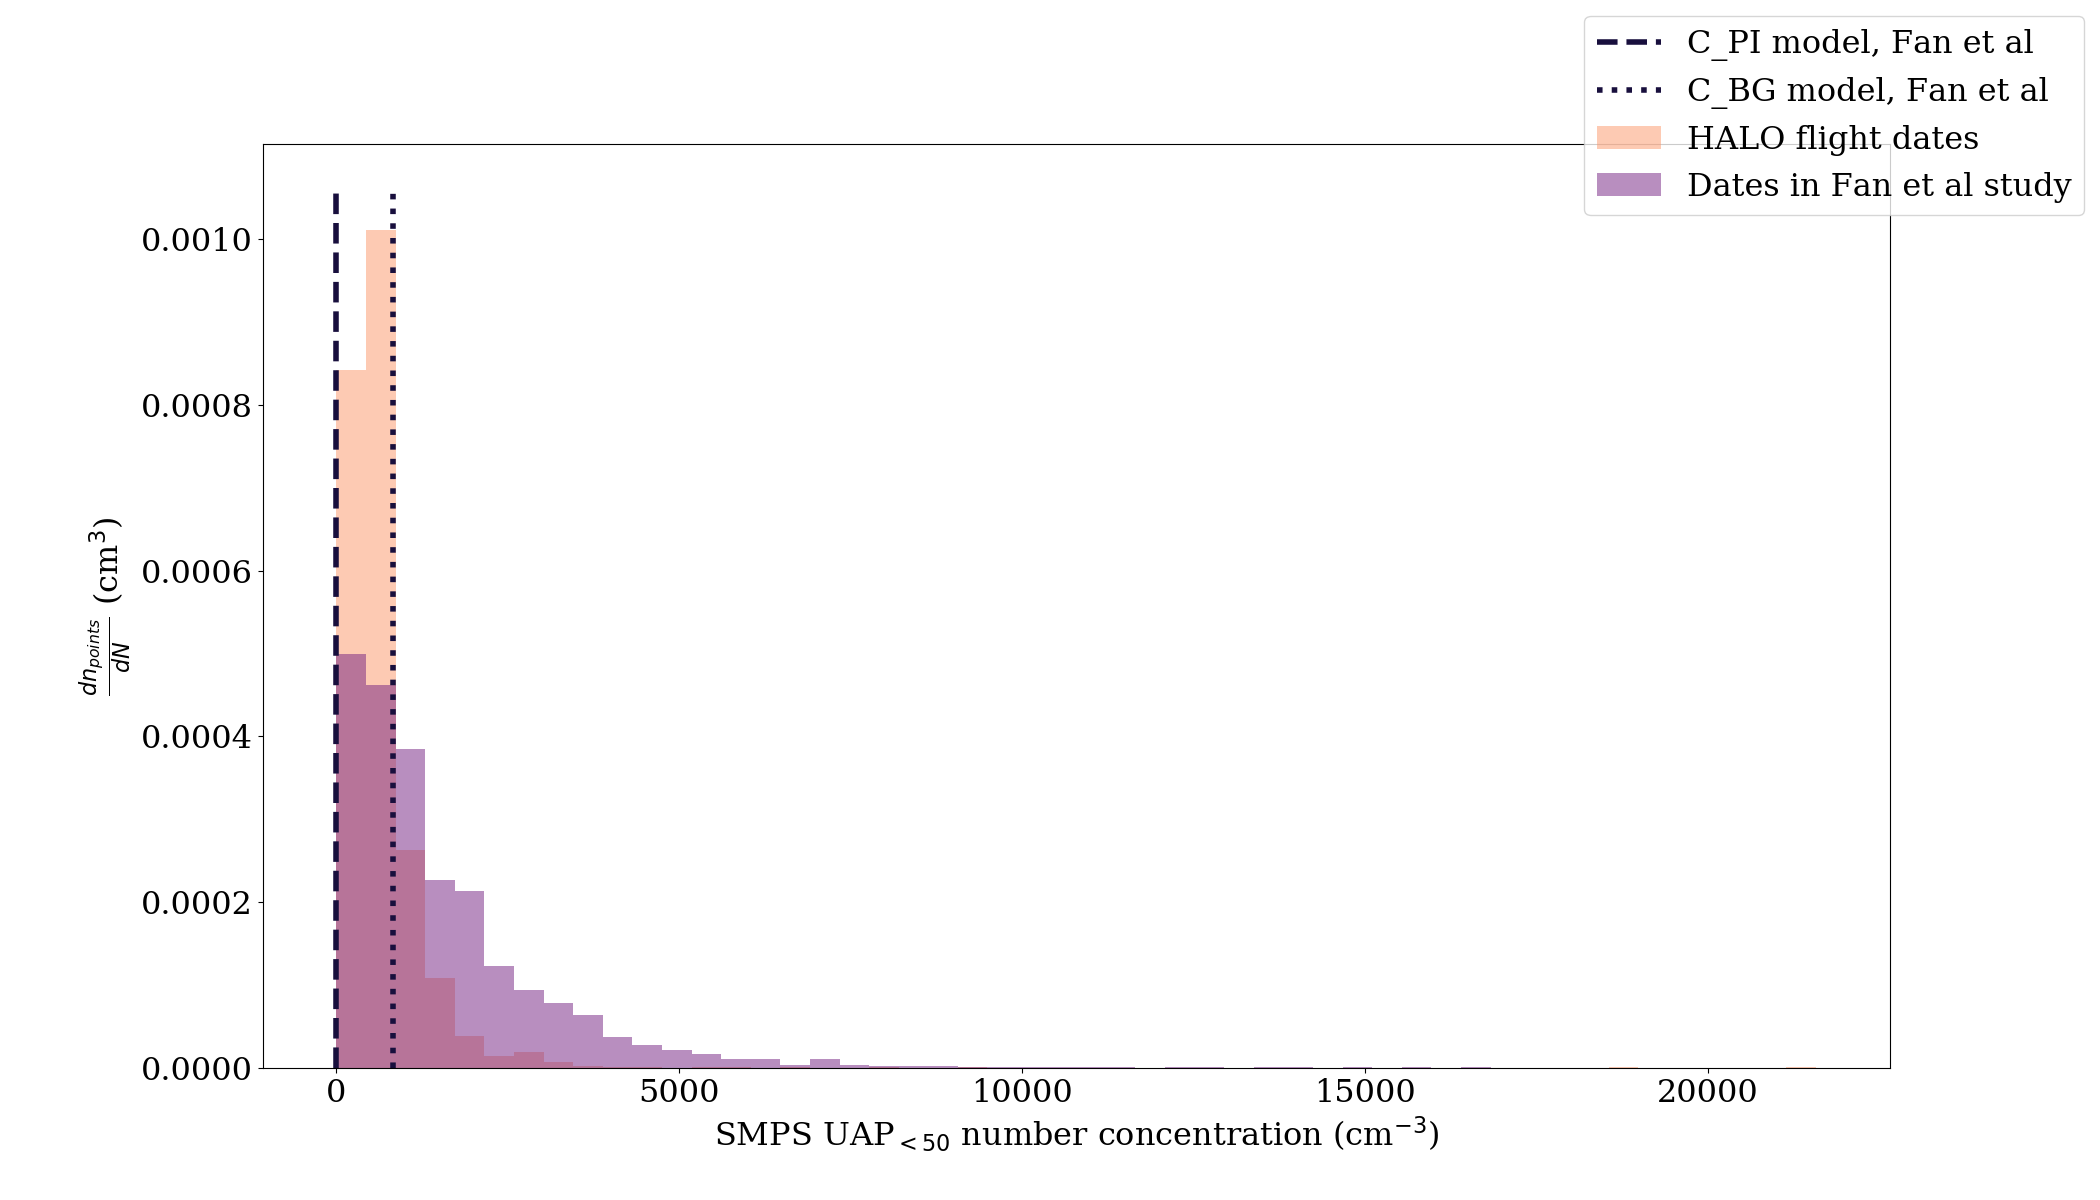
\includegraphics[width=\textwidth]{goama/v1_FINAL_uap50_compare_nconc_hist_alldates_figure.png}
		\label{goamazonuap50hist}
		\caption{}
	\end{subfigure}
	\caption{Distribution of aerosol concentration measurements by the ground-based SMPS at Manacapuru, Brazil; a) entire size range, b) only particles with diameter greater than 50nm. HALO flight dates are the same as those represented in Figure \ref{halossvertprof} (see main text for details). Dashed (dotted) lines show initial concentrations in the BL of the WRF simulation of polluted (unpolluted) conditions. The unpolluted model aerosol concentrations are quite low relative to what is actually observed.}
	\label{goamazonhist}
\end{figure}

Another possible counterargument is that the flight campaigns simply didn't fly through strong enough updrafts. However the vertical velocity distributions from the campaigns are quite similar to that from the simulations. See Figure \ref{combinedwhist}. 

\begin{figure}[ht]
    \centering
    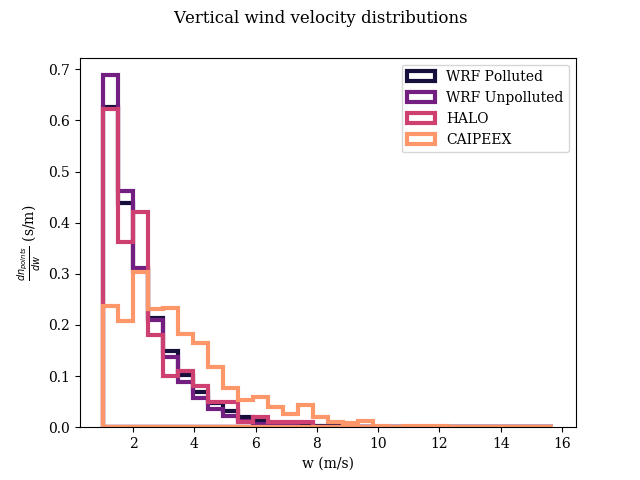
\includegraphics[width=12cm]{wrf/combined_w_hist_figure.png}
    \caption{Vertical wind velocity probability distributions from simulations and field campaigns, using filtering criteria outlined in the text. Experimental distributions are not qualtitatively different from those in the simulation.}
    \label{combinedwhist}
\end{figure}

In order to probe more precisely why the SS profiles for HALO and WRF are so different, we compare their average water drop spectra over the altitude range of 1.5-2.5 km. This range was chosen because it gives a relatively local snapshot while still including a statistically meaningful number of WCU points from the HALO dataset (114 out of 203 total). Figure \ref{combineddsds} a and b show the drop size and mass distributions which determine, respectively, the magnitudes of $SS_{QSS}$ and $LWC$. 

Figure \ref{combineddsds} a is consistent with the order-of-magnitude difference between the average $SS_{QSS}$ values for this altitude slice (0.14\% for HALO, 1.2\% (polluted) and 2.4\% (unpolluted) for WRF) since, from Equation \ref{fullss}, average $SS_{QSS}$ is inversely proportional to the average value of $\sum\limits_{i}r_if(r_i)N(r_i)$ (up to some non-local cross terms in the average which we find contribute to a fractional error of at most 60\%). 

In both panels a and b of Figure \ref{combineddsds} there is an evident bias in the WRF simulations towards larger water drops. In particular, we note the large $LWC$ contribution from drizzle and rain in the WCU regions. This suggests that ... [\klcomm{I think I still need some verbal discussion about this}]

\begin{figure}[ht]
	\centering
	\begin{subfigure}{0.7\textwidth}
		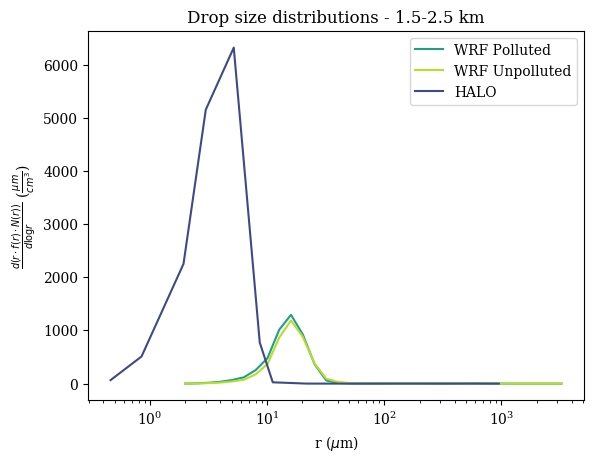
\includegraphics[width=\textwidth]{halo/halo_slice_meanr_dsd_alldates_figure.png}
		\label{combineddsdssize}
		\caption{}
	\end{subfigure}
	\begin{subfigure}{0.7\textwidth}
		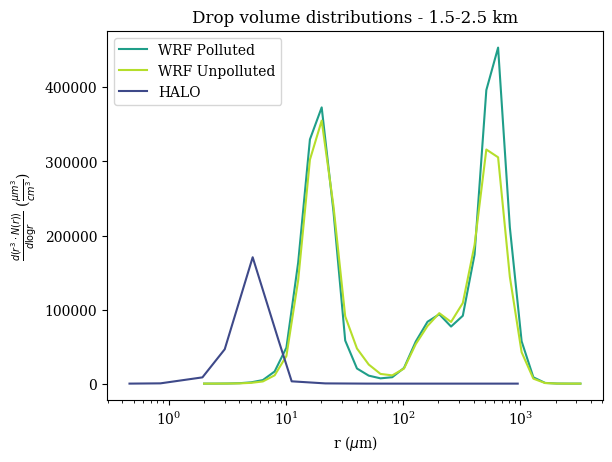
\includegraphics[width=\textwidth]{halo/no_vent_halo_slice_meanr_dsd_alldates_vol_figure.png}
		\label{combineddsdsmass}
		\caption{}
	\end{subfigure}
	\caption{Comparison of water drop spectra in HALO field campaign data versus WRF microphysics simulations; a) size distributions, b) volume distributions. Note that the volume distribution is not weighted by ventilation factor, since we do not use that to calculate $LWC$, and because it artifically inflates the spectrum in the region of higher drop radii. Panel a) is consistent with the discrepancy in derived $SS_{QSS}$ values between experiment and simulation, since the integrated areas of those curves are approximately inversely proportional to $SS_{QSS}$. Panel b) shows more clearly the bias in WRF towards accumulating liquid water in (a relatively small number of) larger drops. [\todo{other comments?}]}
	\label{combineddsds}
\end{figure}

Conclusion: The WPIM as proposed by Fan et al requires the average temperature profile of the troposphere to be set by relatively clean (high-SS) convection, in order for more polluted (low-SS) convection to experience an enhancement in buoyancy. However, we find no evidence that the high SS values reported by Fan's model actually occur in nature, which weakens the possibility of measureable invigoration effects - in particular, we estimate an upper bound on vertical velocity enhancement of $\approx$ 1 m/s from the HALO flight campaign, compared to $\approx$ 10 m/s from Fan's control simulations in WRF. The relatively low aerosol concentrations used to initialize the simulations, in combination with possible irregularities in microphysical parameterizations, may be to blame for the anomalously high SS values in the WRF output.

\clearpage
\newpage

\section{Methods}

\subsection{WRF}

Model output for control simulations of polluted (``C\_BG") and unpolluted (``C\_PI") scenarios were provided by Fan et al; see that paper and accompanying SI for detailed explanations of model parameters and initializations.

In this paper, we use the following form of the QSS SS equation after \cite{Rogers1989} (with $SS_{QSS}$ given as a percentage):
\begin{equation}
\label{fullss}
SS_{QSS} = \frac{A(T) w}{4\pi B(\rho_a, T) \langle f(r)\cdot r\rangle n}*100,
\end{equation}
where:
\begin{align}
A(T) &= \frac{g}{R_a T}\Big(\frac{L_v R_a}{C_{ap} R_v T} - 1\Big)\big(F_d(T) + F_k(T)\big)\nonumber\\
F_d(T) &= \frac{\rho_w R_v T}{D e_s(T)}\nonumber\\
F_k(T) &= \Big(\frac{L_v}{R_v T} - 1\Big)\frac{L_v \rho_w}{K T}\nonumber\\
B(\rho_a, T) &= \rho_w\Big(\frac{R_v T}{e_s(T)} + \frac{L_v^2}{R_v C_{ap} \rho_a T^2}\Big)
\end{align}
Notation for constants and variables is given in Table \ref{vartable}. We use the following parameterization for $e_s$ \cite{Rogers1989}:
\begin{equation}
e_s(T) = 611.2e^{\frac{17.67T_c}{T_c + 243.5}},
\end{equation}
where $T_c$ is the temperature in degrees Celsius.

We note that this equation by also include finite size correction terms; however, using typical values for droplet salinity and condensation nucleus radius (the relevant parameters in this case), these terms are insignificant ($<$ 0.1\% correction to SS) for drops of radius greater than 3 $\mu$m \cite{Rogers1989}, and we therefore do not consider them in this paper.

A simpler form of Equation \ref{fullss} is often employed in the literature \cite{Grabowski2020, Rogers1989}, with:
\begin{align}
A(T) &= \frac{g}{R_a T}\Big(\frac{L_v R_a}{C_{ap} R_v T} - 1\Big)\nonumber\\
B(T) &= D
\end{align}
Figure \ref{simpleqsswrfvsqss} shows that this form does not yield as good of agreement with the actual SS reported in WRF.

We use the expressions given in \cite{Pruppacher2010} and \cite{Rogers1989} for ventilation corrections, which are quite extensive. Full formulae are contained in the analysis code at \href{https://github.com/kt-latimer/20supersat}{this GitHub repo}. Figures \ref{noventwrfvsqss} and \ref{norainnoventwrfvsqss} show, respectively, the effects of neglecting these corrections (i.e. setting $f(r)=1$ for all $r$) for rain drops (defined here as liquid water drops with radius greater than 102 $\mu$m), and omitting rain drops altogether from the calculations of mean radius and number concentration.

\subsection{HALO}

The HALO aircraft supported two instruments for measuring cloud droplet spectra: a cloud and aerosol spectrometer (CAS-DPOL) and a cloud droplet probe (one element of a cloud combination probe) (CCP-CDP) \cite{Braga2017}. We found that the CCP-CDP consistently reported unphysical bimodal size distributions, and therefore used only data from the CAS-DPOL for all calculations involving cloud droplets. Number concentrations from the CAS-DPOL were corrected using the $\xi$ factor derived in \cite{Weigel2016}.

The rain drop spectra came from data collected by greyscale cloud imaging probe (second element of the cloud combination probe) (CCP-CIP). The drop diameter detection ranges for CAS-DPOL and CCP-CIP were 0.89-50 $\mu$m and 25-2000 $\mu$m, respectively. Per guidance from the principal investigators for the CAS-DPOL, we only included data for droplets from size bins with a lower diameter bound greater than or equal to 3 $\mu$m in the analysis \cite{Jurkat2020}.  

There was some ambiguity in how to treat the region of overlap of the CAS-DPOL and the CCP-CIP instruments. Upon examination of spectra across the range of dates in question, we see that the first size bin for CCP-CIP consistently reports suspect measurements. For example, correlation in number concentrations measured by this bin with those measured by neighboring bins is consistently low (Figure \ref{cipbin1corr}), and there are a relatively high number of instances where the spectrum shows an unphysical spike for that bin (Figure \ref{cipbin1anom}). We therefore apply the average value of $\frac{dN}{dlogDp}$ for all CAS-DPOL bins in the range of 25-50 $\mu$m diameter across the entire region of 25-75 $\mu$m diameter (namely the range of CCP-CIP bin 1). 

All measurements of environmental variables were taken from the Basic Halo Measurement and Sensor System (BAHAMAS).

Out of the dates for which all three instruments (BAHAMAS, CAS-DPOL, CCP-CIP) report data, we take those for which measurements of shared variables (true airspeed for BAHAMAS and CAS-DPOL; $\xi$ correction factor for CAS-DPOL and CCP-CIP) are well-correlated ($R^2$ above 0.95). These are (all in 2014): 6, 9, 11, 12, 16, 18, 27, 28, 30 September; 1 October (a total of 10 dates out of 14 total for HALO in the ACRIDICON-CHUVA campaign). See \cite{Wendisch2016} for a map of flight tracks on each individual day.

\klcomm{You listed a few more seeminly very basic questions but it's ambiguous how to quantitatively answer them, and part of the reason I'm struggling to do so in this case is that I have no idea why or in what context a typical reader would want to know these things. Here are some vaguely structured thoughts and ideas:}
\begin{itemize}
\item \drcomm{How did they select clouds to fly through?} \klcomm{As described in Wendisch 2016, there were five different research topics (`Cloud vertical evolution and life cycle (cloud profiling)', `Cloud processing of aerosol particles and trace gases (inflow and outflow)', etc) that determined the vertical flight profiles. In this paper they mention flying through specific types of clouds for some of the research topics...is this something we need to reiterate ourselves? For further context, the dates I chose include at least one flight for each of the five topics.}
\item \drcomm{Over what duration in time are the data for your calculation collected?} \klcomm{Are you asking how long the flights lasted? Total flight times lasted between 5-8 hours each, but I'm just taking out sporadic snippets...is the relevant information like the fraction of data points (i.e. flight time) that I use after filtering? Or is it the average time spanned by consecutive points passing through the filter? In short, what is the physical meaning of the time scale we're looking for.}
\item \drcomm{Over what distance are those data averaged?} \klcomm{Basically the same as above...is this the total distance traveled over the course of the flight, the average distance travelled between samples, the average size of cloudy regions?}
\end{itemize}

We used the same Equation \ref{fullss} for $SS_{QSS}$ and for ventilation factors as described above.

\clearpage
\newpage

\section{Supplementary}

\begin{figure}[ht]
	\centering
	\begin{subfigure}{0.7\textwidth}
		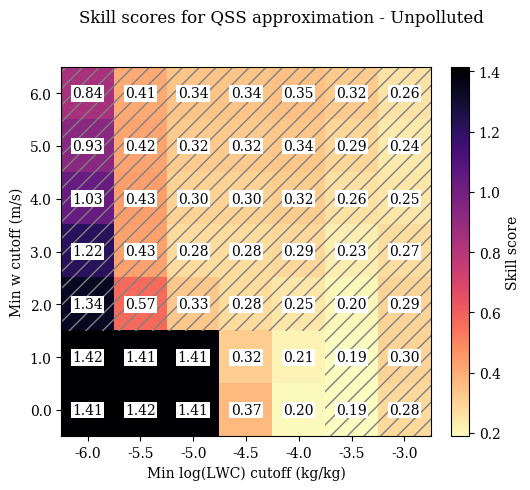
\includegraphics[width=\textwidth]{wrf/filtering_criteria_separate_Unpolluted_figure.png}
		\caption{Unpolluted case.}
		\label{filtcritheatmapsepunpoll}
	\end{subfigure}
	\begin{subfigure}{0.7\textwidth}
		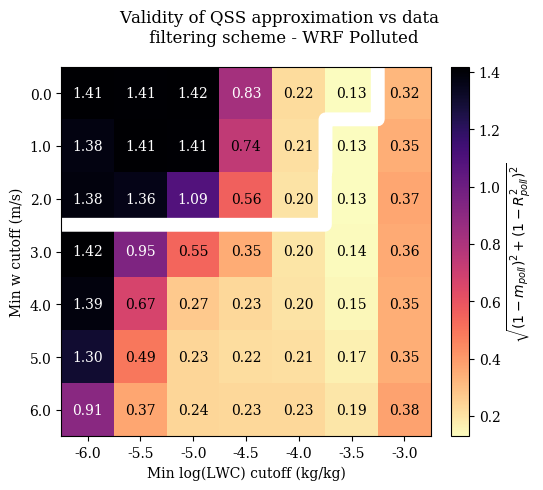
\includegraphics[width=\textwidth]{wrf/filtering_criteria_separate_Polluted_figure.png}
		\caption{Polluted case.}
		\label{filtcritheatmapseppoll}
	\end{subfigure}
	\caption{Same as Figure \ref{filtcritheatmap}, but separated by simulation case (polluted and unpolluted, or `C\_BG and' `C\_PI' in Fan et al). In both panels, the skill score is defined as the Euclidean distance between $(m, R^2)$ where $m$ and $R^2$ are LSLR parameters from fitting $SS_{WRF}$ vs $SS_{QSS}$ and the ideal point (1, 1).}
	\label{filtcritheatmapsep}
\end{figure}

\begin{figure}[ht]
	\centering
	\begin{subfigure}{0.7\textwidth}
		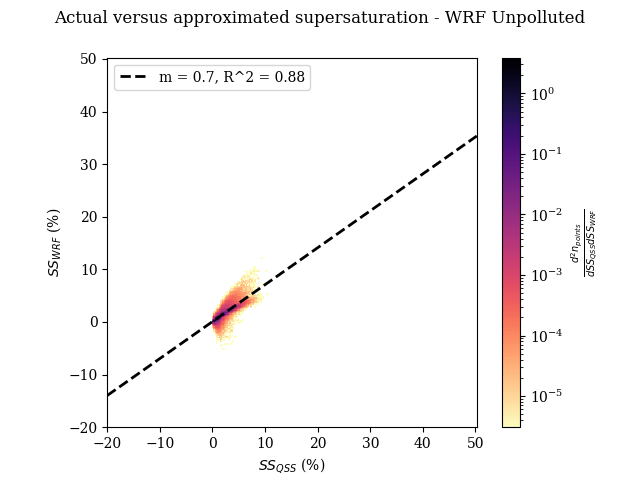
\includegraphics[width=\textwidth]{wrf/heatmap_ss_qss_vs_ss_wrf_Unpolluted_figure.png}
		\caption{Unpolluted case.}
		\label{wrfvsqssunpoll}
	\end{subfigure}
	\begin{subfigure}{0.7\textwidth}
		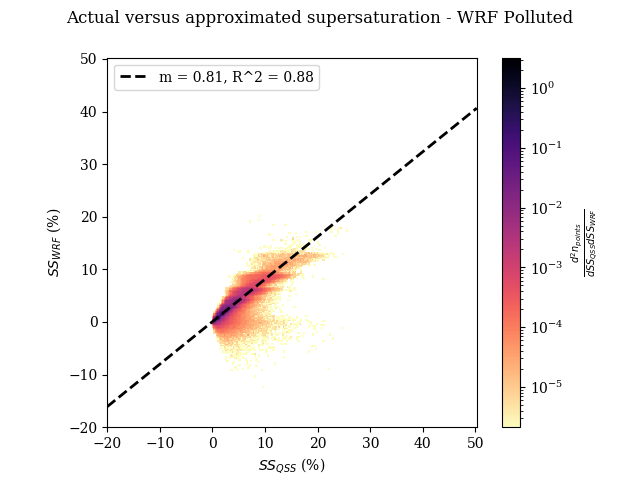
\includegraphics[width=\textwidth]{wrf/heatmap_ss_qss_vs_ss_wrf_Polluted_figure.png}
		\caption{Polluted case.}
		\label{wrfvsqsspoll}
	\end{subfigure}
	\caption{Plot of $SS_{QSS}$ versus $SS_{WRF}$ using the filtering scheme described in the main text. Dashed line shows the fit from LSLR. Color denotes the density of data points; note the scale is logarithmic in this figure. The majority of points are clustered near the origin.}
	\label{wrfvsqss}
\end{figure}

\begin{figure}[ht]
	\centering
	\begin{subfigure}{0.7\textwidth}
		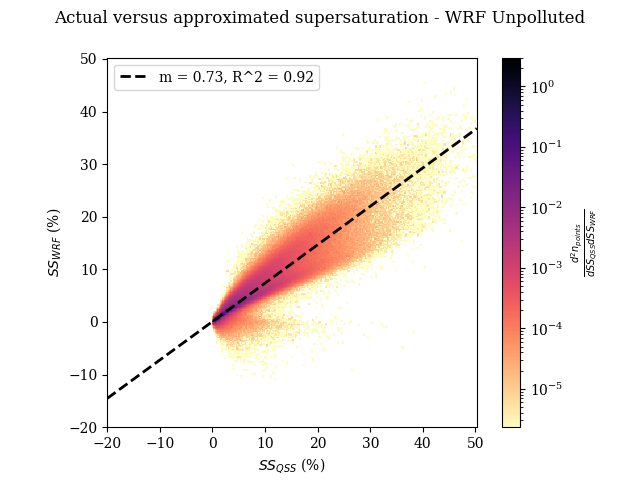
\includegraphics[width=\textwidth]{wrf/simpleqss_heatmap_ss_qss_vs_ss_wrf_Unpolluted_figure.png}
		\caption{Unpolluted case.}
		\label{simpleqsswrfvsqssunpoll}
	\end{subfigure}
	\begin{subfigure}{0.7\textwidth}
		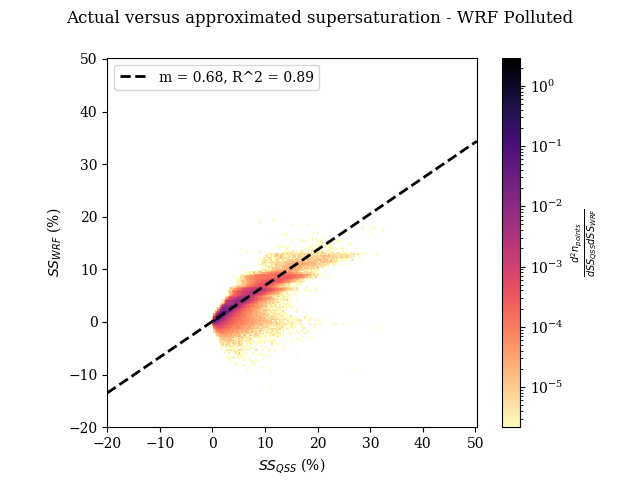
\includegraphics[width=\textwidth]{wrf/simpleqss_heatmap_ss_qss_vs_ss_wrf_Polluted_figure.png}
		\caption{Polluted case.}
		\label{simpleqsswrfvsqsspoll}
	\end{subfigure}
	\caption{Same as Figure \ref{wrfvsqss}, using simplified form of Equation \ref{fullss}. Correlation is not appreciably affected but the value of LSLR slopes is lower for both simulation cases.}
	\label{simpleqsswrfvsqss}
\end{figure}

\begin{figure}[ht]
	\centering
	\begin{subfigure}{0.7\textwidth}
		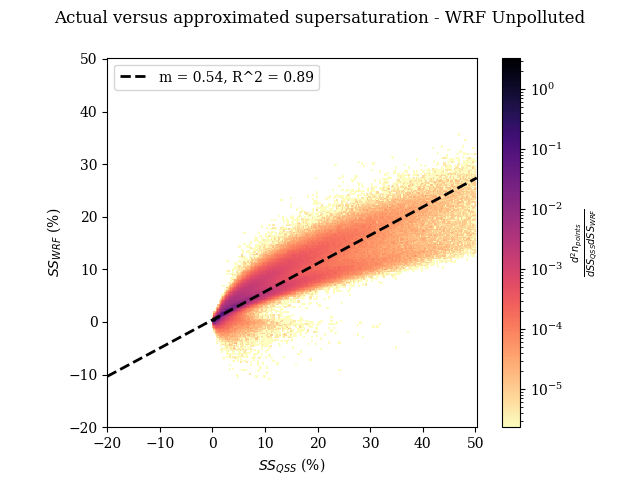
\includegraphics[width=\textwidth]{wrf/novent_heatmap_ss_qss_vs_ss_wrf_Unpolluted_figure.png}
		\caption{Unpolluted case.}
		\label{noventwrfvsqssunpoll}
	\end{subfigure}
	\begin{subfigure}{0.7\textwidth}
		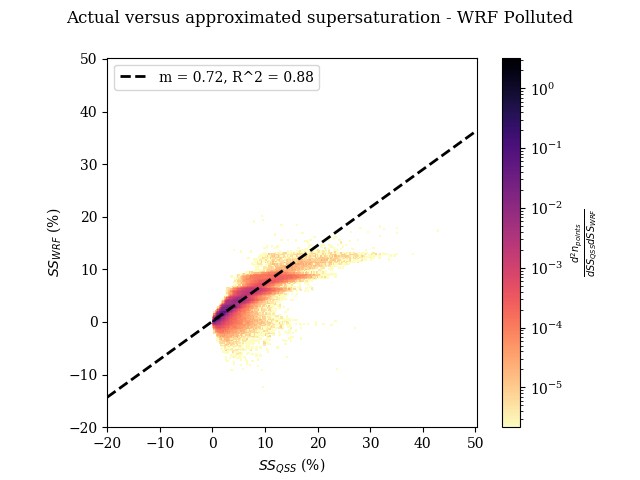
\includegraphics[width=\textwidth]{wrf/novent_heatmap_ss_qss_vs_ss_wrf_Polluted_figure.png}
		\caption{Polluted case.}
		\label{noventwrfvsqsspoll}
	\end{subfigure}
	\caption{Same as Figure \ref{wrfvsqss}, without ventilation corrections. Correlation is not appreciably affected but the value of LSLR slopes is lower for both simulation cases.}
	\label{noventwrfvsqss}
\end{figure}

\begin{figure}[ht]
	\centering
	\begin{subfigure}{0.7\textwidth}
		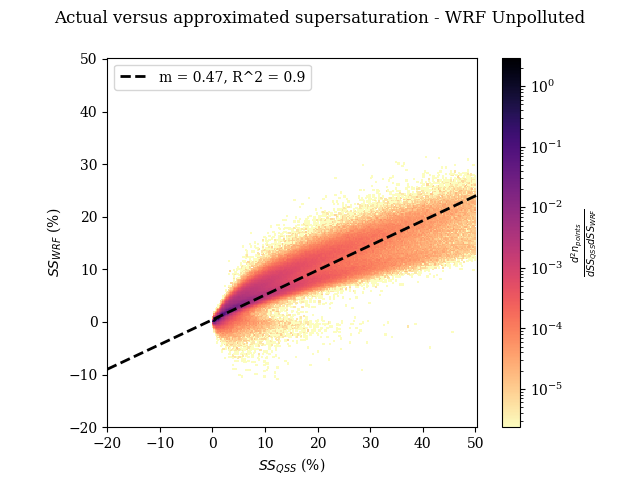
\includegraphics[width=\textwidth]{wrf/norainnovent_heatmap_ss_qss_vs_ss_wrf_Unpolluted_figure.png}
		\caption{Unpolluted case.}
		\label{norainnoventwrfvsqssunpoll}
	\end{subfigure}
	\begin{subfigure}{0.7\textwidth}
		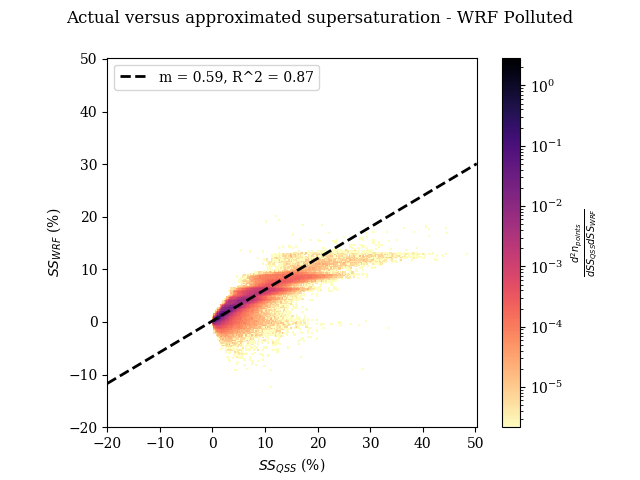
\includegraphics[width=\textwidth]{wrf/norainnovent_heatmap_ss_qss_vs_ss_wrf_Polluted_figure.png}
		\caption{Polluted case.}
		\label{norainnoventwrfvsqsspoll}
	\end{subfigure}
	\caption{Same as Figure \ref{wrfvsqss}, without contributions from rain drops. Correlation is slightly lower and the value of LSLR slopes is lower for both simulation cases.}
	\label{norainnoventwrfvsqss}
\end{figure}

\begin{figure}[ht]
	\centering
	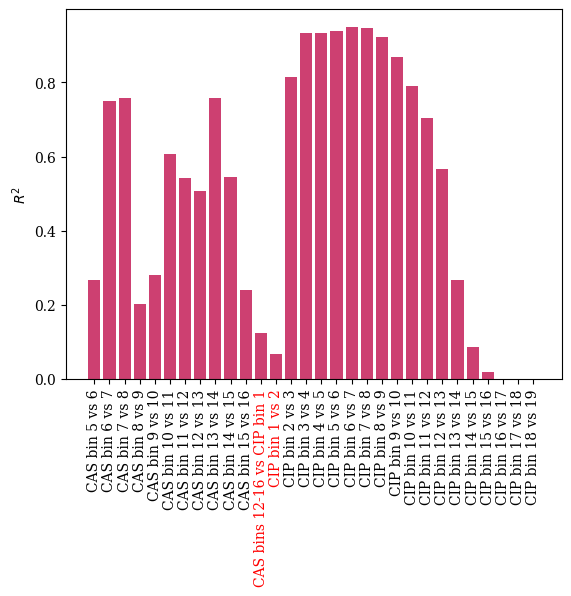
\includegraphics[width=\textwidth]{halo/bin_correlations_figure.png}
	\caption{Correlation coefficient for number concentrations measured in adjacent or overlapping bins. We find that number concentrations measured by CCP-CIP bin 1 (25-75 $\mu$m diameter) correlate poorly with those measured by CAS bins 12-16 (25-50 $\mu$m diameter) and by CIP bin 2 (75-125 $\mu$m diameter), indicating discontinuity with the rest of the drop size distribution at that point. The very low correlations at the upper end of the total size range are due to the fact that number concentrations in that regime are very close to zero for all times and therefore are essentially noise.}
	\label{cipbin1corr}
\end{figure}

\begin{figure}[ht]
	\centering
	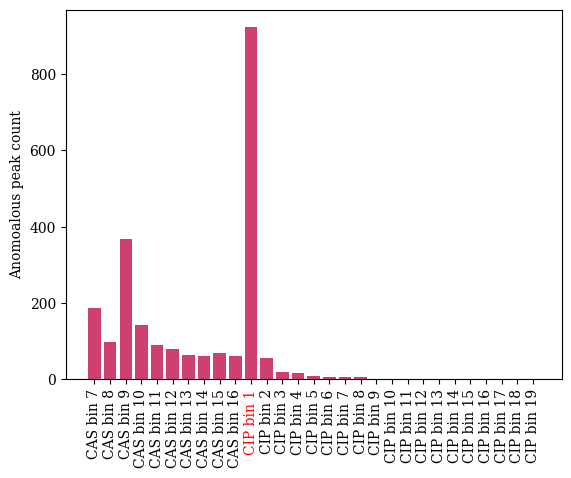
\includegraphics[width=\textwidth]{halo/v2_anomalous_spectrum_counts_figure.png}
	\caption{Raw count of samples across all dates under consideration where $\frac{dN}{dlogDp}$ measured by a given bin is a global maximum for the spectrum and also greater than 5 times the next highest bin's $\frac{dN}{dlogDp}$ in that same spectrum. This figure shows that the measured spectrum often has a spike at CIP bin 1, which we believe is unphysical.}
	\label{cipbin1anom}
\end{figure}

\begin{figure}[ht]
	\centering
	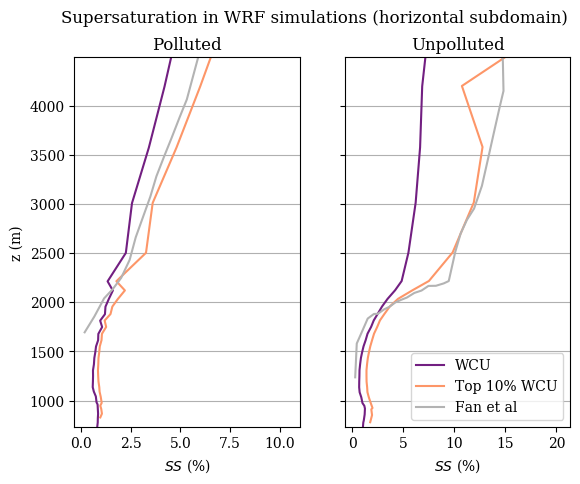
\includegraphics[width=\textwidth]{wrf/subdom_ss_pred_vs_z_figure.png}
	\caption{Analagous to Figure \ref{wrfssvertprof}, restricted to the horizontal subdomain indicated by the red box in Figure S8 of Fan et al (bottom left panel). Qualitatively the results are quite similar, suggesting that the restriction to this subdomain is not crucial to the results described in Fan's paper.}
	\label{wrfsubdomssvertprof}
\end{figure}

\begin{sidewaystable}[]
\centering
\begin{tabular}{@{}llll@{}}
\toprule
Symbol & Meaning & Value of constant & Notes \\ \midrule
$C_{ap}$ & Specific heat capacity at constant pressure, dry air & 1005 J/kg &  \\
$D$ & Molecular diffusion constant of water in dry air & 0.23e-4 m$^2$/s & We take as constant wrt T \\
$e_s$ & Saturation vapor pressure, water & - &  \\
$f(r)$ & Ventilation factor & - &  \\
$g$ & Gravitational acceleration on Earth & 9.8 m/s &  \\
$K$ & Coefficient of thermal conductivity in dry air & 2.4e-2 J/(m s K) & We take as constant wrt T \\
$LWC$ & Liquid water content & - &  \\
$L_v$ & Latent heat of vaporization, water & 2.501e6 J/kg & We take as constant wrt T \\
$N$ & Particle number concentration & - &  \\
$n_{points}$ & Point probability density & - &  \\
%$N_{points}$ & Absolute number of points & - &  \\
$q_v$ & Water vapor mass mixing ratio & - & Equals $\frac{m_v}{m_{tot}}$ \\
$q_v^*$ & Saturation water vapor mass mixing ratio & - & Equals $\frac{m_v^*}{m_{tot}}$ \\
$r$ & Particle radius & - &  \\
$RH$ & Relative humidity & - & Equals $SS+1$ \\
$\rho_a$ & Mass density, dry air & - & Assuming ideal gas law \\
$\rho_w$ & Mass density, liquid water & 1000 kg/m$^3$ &  \\
$R_a$ & Ideal gas constant, dry air & 287.19 J/(kg K) &  \\
$R_v$ & Ideal gas constant, water & 460.52 J/(kg K) &  \\
$SS$ & Supersaturation & - & Equals $RH-1$ \\
$T$ & Temperature & - &  \\
$T_c$ & Temperature in degrees C & - & Equals $T – 273.15$ \\
$w$ & Vertical wind velocity & - &  \\
$z$ & Altitude & - &  \\ \bottomrule
\end{tabular}
\caption{Explanation of constants and variables used in the paper.}
\label{vartable}
\end{sidewaystable}

\clearpage
\newpage

\bibliography{refs}
\bibliographystyle{ieeetr}
\end{document}
